\documentclass[float=false, crop=false]{standalone}
\usepackage[subpreambles=false]{standalone}
\usepackage{import}

\usepackage{subfiles}
\usepackage[backend=biber,style=numeric,sorting=none]{biblatex}
\usepackage[pdfborder={0 0 0}]{hyperref}   
\usepackage[margin=25mm]{geometry} 
\usepackage{graphicx}  
\usepackage[utf8]{inputenc}
\usepackage{textcomp}
\usepackage{import}
\usepackage[font=small,labelfont=bf]{caption}

\usepackage{stmaryrd}
\usepackage{verbatim}
\usepackage{amsmath}
\usepackage{amsfonts}
\usepackage{amssymb}
\usepackage{amsthm}
\usepackage{sansmath}
\usepackage{mathtools}

\usepackage{pgfgantt}
\usepackage{graphicx}
\usepackage{xcolor}

\ganttset{group/.append style={orange},
          milestone/.append style={red},
          progress label node anchor/.append style={text=red}}

\usepackage{color}

\newlength\gwidth
\newlength\gheight
\setlength{\gwidth}{\textwidth}
\setlength{\gwidth}{\textheight}

\newcommand{\namefig}{\textbf{Figure}~}

\definecolor{pblue}{rgb}{0.13,0.13,1}
\definecolor{pgreen}{rgb}{0,0.5,0}
\definecolor{pred}{rgb}{0.9,0,0}
\definecolor{pgrey}{rgb}{0.46,0.45,0.48}

\usepackage{listings}
\lstnewenvironment{JavaLst}
{\lstset{language=Java,
  showspaces=false,
  showtabs=false,
  breaklines=true,
  showstringspaces=false,
  breakatwhitespace=true,
  commentstyle=\color{pgreen},
  keywordstyle=\color{pblue},
  stringstyle=\color{pred},
  basicstyle=\ttfamily,
  moredelim=[il][\textcolor{pgrey}]{$$},
  moredelim=[is][\textcolor{pgrey}]{\%\%}{\%\%},
  escapeinside={&}{&}
}}{}

\lstnewenvironment{HaskellLst}
{\lstset{
  frame=none,
  xleftmargin=2pt,
  stepnumber=1,
  numbersep=5pt,
  numberstyle=\ttfamily\tiny\color[gray]{0.3},
  belowcaptionskip=\bigskipamount,
  commentstyle=\color{pgreen},
  keywordstyle=\color{pblue},
  stringstyle=\color{pred},
  basicstyle=\ttfamily,
  captionpos=b,
  escapeinside={*'}{'*},
  language=haskell,
  tabsize=2,
  emphstyle={\bf},
  commentstyle=\it,
  showspaces=false,
  columns=flexible,
  showstringspaces=false,
  morecomment=[l]\%,
}} {}

\lstnewenvironment{JVMLst}
{\lstset{
  frame=none,
  numbers=none,
  xleftmargin=2pt,
  language=JVMIS,
  emphstyle={\bf},
  stringstyle=\mdseries\rmfamily,
  commentstyle=\color{pgreen},
  stringstyle=\color{pred},
  keywordstyle=\color{black},
  basicstyle=\ttfamily,
  basicstyle=\small\sffamily
}} {}

\usepackage{tikz}
\usetikzlibrary{positioning}

\tikzset{
  treenode/.style = {shape=rectangle, rounded corners,
                     draw, align=center,
                     top color=white, bottom color=blue!20},
  root/.style     = {treenode, font=\ttfamily\Large},
  env/.style      = {treenode, font=\ttfamily\normalsize},
  dummy/.style    = {circle,draw}
}

\newcommand{\tlang}{\star}
\newcommand{\thunk}[1]{\lceil #1 \rceil}
\newcommand{\unwrap}[1]{\lfloor #1 \rfloor}
\newcommand{\tcbn}{\rightarrow_N}
\newcommand{\tcbv}{\rightarrow_V}
\newcommand{\tccbv}{\rightarrow_V^*}
\newcommand{\tthunk}{\rightarrow_\tlang}
\newcommand{\tlthunk}{\rightsquigarrow_\tlang}

\begin{document}

\section{Overview}
% A functional compiler is usually though of as a five stage pipeline consisting of:

% \begin{enumerate}
%   \item Lexing and Parsing.
%   \item Desugaring.
%   \item Type Checking.
%   \item Optimisation.
%   \item Code Generation.
% \end{enumerate}
% This is how I will split up the implementation of the compiler.

% \section{Lexing and Parsing}

% Parsing and lexing of programming is a well research problem with 
% powerful tools that can be used to implemented a lexer and parser, so
% will details will be given of this stage when compared to others.


% The Haskell 98 report \cite[2.]{haskell98-spec} provides a full specification
% of lexing rules, I implemented a subset of these rules using 
% Alex\cite{alex-lib}. This transform will go from a input text to a set
% of lexical tokens. These tokens are expressed using the data type
% \texttt{LToken}.

% The Haskell 98 report \cite[3.]{haskell98-spec} provides a full specification
% of parsing rules, which again I implemented a subset of, this time using
% the parsing generator Happy\cite{happy-lib}.

\section{Work division}

A waterfall model was used to develop the compiler, since I was the only 
person working on the compiler. This resulted in a linear ordering to work packages being
completed. \namefig\ref{figure:ganttchar} shows how to project progressed. The first
few weeks matched up to the proposed timetable given the project proposal, however implementing
the type inference (TI) was quicker than expected meaning that the only slack given (over the Christmas
holidays) was not needed and I started work on future work projects. The slack time was very generous, if 
without the slack time this project would have been delivered only one week early.

\subimport{workStages/}{workStageGantt.tex}

\section{Lexing and Parsing}

\begin{itemize}
  \item Maybe show a small subset of the grammar and expression and how
    that can be implemented in Alex and Happy. 

  \item Talk about how it can be implemented as an LR(0) parser.
\end{itemize}

\section{Desugaring}

\begin{itemize}
  \item Talk about kind inference, this can be related closely to 
    TI, so used a very similar method as used in TI.

  \item Maybe talk about simple different between desugared before and after.

  \item Talk about build-in data types being added to the desugaring.

\end{itemize}

\section{Type Inference}

The type inference stage in JVHC was heavily influenced by a paper
called `Typing Haskell in Haskell'\cite{thih}. This paper laid 
out an implementation in Haskell of how to run type inference
over a whole Haskell program was finding the type of each definition.
I will therefore not go into detail about the implementation of the 
type inference itself. I will however talk about moving from a Haskell
syntax tree to a valid system F like core language.
This process was interlaced with the type inference algorithm.
This means the result of running type inference gave a type for each
top level function, and also a new data type called \texttt{CoreExpr}

The full CoreExpr datatype is listed in \namefig\ref{code:CoreExpr}. 
All the types in this datatype
are directly from System F, apart from case which was defined above.
The data type is parameterised on \texttt{b}, this is a binder type which 
only stores the variable name and type.


\begin{figure}
  \centering
  \begin{lstlisting}[language = Haskell, escapechar = !]
        data Expr b
          = Var  Id
          | Lit  Literal
          | App  (Expr b)     (Arg  b)!
          \tikz[remember picture] \node [] (arg) {};
          !
          |!
           \tikz[remember picture] \node [] (lam) {};
         !Lam  b            (Expr b)
          | Let  (ExprDef b)  (Expr b)
          | Case (Expr b)     Type     [Alt b]!
          \tikz[remember picture] \node [] (alts) {};
          !
          |!
          \tikz[remember picture] \node [] (type) {};
          !Type Type

        data ExprDef b = ExprDef b (Expr b)
  \end{lstlisting}
  \begin{tikzpicture}[remember picture, overlay,
    every edge/.append style = { ->, thick, >=stealth,
                                   dashed, line width = 0.5pt },
    every node/.append style = { align = center, minimum height = 10pt,
                                 font = \bfseries, fill={rgb:black,1;white,20}},
                  text width = 2.5cm ]
  \node [left = 0.5 cm of lam,text width = 2.2cm]
                             (Lam) {Could be $\Lambda$ or $\lambda$.};
  \node [right = 0.5 cm of arg,text width = 2.2cm]
                             (Arg) {Could be a \texttt{Expr} or a \texttt{Type}.};
  \node [right = 0.5 cm of alts,text width = 2.2cm]
                             (Alts) {List of possible branches.};
  \node [left = 0.5 cm of type,text width = 2.2cm]
                             (Type) {Types erased for code gen.};
  \draw (Lam.east)  + (0, 0) coordinate(x1) edge (lam.east|-x1);
  \draw (Arg.west)  + (0, 0) coordinate(x1) edge (arg.west|-x1);
  \draw (Alts.west) + (0, 0) coordinate(x1) edge (alts.west|-x1);
  \draw (Type.east) + (0, 0) coordinate(x1) edge (type.east|-x1);
\end{tikzpicture} 
  \caption[Listing of \texttt{CoreExpr} data type]{Listing of \texttt{CoreExpr} data type. The \texttt{Type} type represents any possible type, this 
  is the same type as in the type inference section above}
  \label{code:CoreExpr}
\end{figure}
The resulting code returned from the mixed type inference and syntax transform stage was not quite
valid \texttt{CoreExpr}. To convert this resulting syntax tree to valid System F, type information
need be added explicitly, this meant adding both type applications and $\Lambda$ (type abstractions)
to the syntax. To add these constructs a lookup table was also returned to the type inference stages, 
which contained the type of every sub-expression. This was used to insert type applications and
$\Lambda$ in the correct places in the syntax tree making the resulting syntax tree valid again.

% \begin{itemize}
%   \item Talk about paper.

%   \item Talk about understanding the paper

%   \item Talk about modification I made to remove type classes.

%   \item Talk about going to the broken core output
%     from TI, to valid system F in the form with all $\Lambda$ at the 
%     start of the expression and with the correct inserted types.

%   \item Talk about build in functions being added to the TI.
% \end{itemize}

\section{Inlining}

% \begin{itemize}
%   \item Talk about general principle a bit.

%   \item Talk about the inline monad and the \texttt{inline} function
%     and the \texttt{rename} function and monad.

%   \item Talk about when to inline, don't inline recursive functions.
%     Be careful inlining \texttt{id x = id x}.

%   \item Talk about inline metric to decide whether a function should be inlined.
% \end{itemize}

Functional inlining, comes from the idea that it 
would be better to inline some function, so 
to remove the need for the function call to happen, 
also if a function has been inlined, this might allow further
inlining to occur, such as constant folding.

Constant folding is replacing a branch instruction
(in Haskell a \verb|case| expression), where the outcome is 
known at compile time with the code for that branch only.

First I will explain constant folding in more detail since
it is a more simple concept.

Given an expression 

\begin{HaskellLst}
case 2 of 
  1 -> e
  2 -> e'
\end{HaskellLst}

Using constant folding this expression would be reduced to

\begin{HaskellLst}
e'
\end{HaskellLst}

Functional inlining is more interesting. The technique I used
was heavily influenced by the paper\cite{ghc-inliner}, its 
revolves around when to inline:
\begin{HaskellLst}
let x = e in e'
\end{HaskellLst}
where \verb|e'| contains free references to \verb|x|.
Other parts of the syntax that could be inlined
can instead to written in terms of a \verb|let| construct.

\begin{HaskellLst}
(\x -> e) e'
\end{HaskellLst}
Goes to
\begin{HaskellLst}
let x = e' in e 
\end{HaskellLst}

Now when to inline the \verb|let| construct is a very hard
question to answer. We make sure of two things, one the 
inline must terminate, therefore we cannot inline recursive 
function forever, and two we wish to inlined code to 
performance better (in what ever metric we use) than the original
code.
First I will consider the termination.
This is more easily solved than the second problem.
I simply don't inline any recursive functions.
When trying to answer the question of whether the inlined
code will perform better, there is a load of subtly. First
I will say better means runs faster. Then two thing must
be worked out to decide if inlining is a good idea, first
the code of computing \verb|e'| and second the number of times
\verb|x| appear in \verb|e|. We want the cost of computing
\verb|e'| to be small and the number of times \verb|x| appear
in \verb|e| to also be small. I came up with version simple
metrics
\begin{itemize}
  \item For the cost of \verb|e'| I just assumed it to be constant.
    I is not possible to know the cost at compile time, only
    heuristic could be used. For example if the expression
    \verb|e'| contained any recursive functions
    then have a high cost to compute \verb|e'|.

  \item For the number of times \verb|x| is free in \verb|e'|
    this value can be computed, then I said any time that
    there are four or more free occurrences, don't inline.
    If there are less than four free occurrences then inline.
\end{itemize}

\section{Code Generation}

% \begin{itemize}
%   \item Talk about how each part of the syntax tree was converted from 
%     CoreExpr to classes.

%   \item Link back to original proposal before coding about how to implement
%     everything.

%   \item Talk about verifiable bytecode.

%   \item 
% \end{itemize}

In the preparation section I created a document to mark down the 
translation between the CoreExpr data-type and JVM bytecode instructions.
Code Generation is just finding a correct mapping between \texttt{CoreExpr} defined in 
\namefig\ref{code:CoreExpr}.

After considering the input data \texttt{CoreExpr}, next I considered what the result of each element 
of the data type would map to. I have shown mapping from the \texttt{CoreExpr} data type to
Java code for the reader convenience, however in the compiler the conversion was to JVM bytecode.
This compiler must emulate a computation that can be carried on at a later date. This can be implemented
using thunks. In JVHC this will be implemented by creating a class
which implements a method \verb|force|, \verb|force| will be called by \verb|get| in the default
implementation of a thunk.

\begin{JavaLst}
public abstract class Thunk<T> implements Supplier<T> {
    private T value;
    protected abstract T force();
    @Override
    public T get() {
        if ( value == null ) {
            return value = force();
        }
        return value;
    }
}
\end{JavaLst}

The important part of this implementation is that once force has been called once
the value will be cached inside this class and future calls to \verb|get| will result
in the cached value being returned. The thunk will implement the supplier interface:
\begin{JavaLst}
public interface Supplier<T> { T get(); }
\end{JavaLst}
in the hope of better integration with existing Java 8 functional interfaces

Functions will also implement the Function interface
\begin{JavaLst}
public interface Function<T, R> { R apply(T t); }
\end{JavaLst}
When first implementing code generation there were bugs, in the implementation
where the mapping between \texttt{CoreExpr} and the lazy language implemented
via the use of thunks. Due to this I decided to formalise this translation, 
the result was a mathematical framework for expression both 
\texttt{CoreExpr} and the thunk language called core calculus and 
core calculus$_\star$ respectively. This is included 
Appendix~\ref{appendix:thunkProof}. 
The notation $\thunk{e}$ means, the value $e$ is wrapped in a thunk. Then
$\unwrap{t}$ means, get the value from the thunk $t$. This would mean calling
\texttt{get} in JVM bytecode.
The translation relation $\tlthunk$ from core calculus to core 
calculus$_\star$ is defined as:

\begin{align*}
  &\frac{}{c \tlthunk \thunk{c}}\\ \\
  &\frac{}{x \tlthunk \thunk{x}}\\ \\
  &\frac{e \tlthunk e_\tlang}
     {\lambda x . e \tlthunk \thunk{\lambda x_\tlang.\unwrap{e_\tlang}}}\\ \\
  &\frac{e  \tlthunk e_\tlang \quad e' \tlthunk e'_\tlang}
  {e e' \tlthunk \thunk{\unwrap{e_\tlang} e'_\tlang}}\\ \\
  &\dfrac{e_1  \tlthunk e_{1_\tlang} \quad \dots \quad e_n \tlthunk e_{n_\tlang} \quad e' \tlthunk e_\tlang}
  {\splitdfrac{\mathtt{let}\ (x_1\ \mathtt{=}\ e_1,\dotsc, x_n\ \mathtt{=}\ e_n)\ \mathtt{in}\ e \tlthunk}
    {\thunk{\mathtt{let}\ 
        (x_1\ \mathtt{=}\ e_{1_\tlang},\dotsc, x_n\ \mathtt{=}\ e_{n_\tlang}) \ \mathtt{in}\ \unwrap{e_\tlang}}}}\\ \\
  &\dfrac{e_1  \tlthunk e_{1_\tlang} \quad \dots \quad e_n \tlthunk e_{n_\tlang} \quad e' \tlthunk e'_\tlang}
  {\splitdfrac{\mathtt{case}\ e\ \mathtt{of}\ b_1 \rightarrow e_1; \dots; b_n \rightarrow e_n \tlthunk}
  {\thunk{\mathtt{case}\ \unwrap{e_\tlang}\ \mathtt{of}\ b_1 \rightarrow \unwrap{e_{1_\tlang}}; 
      \dots; b_n \rightarrow \unwrap{e_{n_\tlang}}}}}
\end{align*}

Then from this it can proved in Appendix~\ref{appendix:thunkProof} 
that the call-by-name transition relation that Haskell should implement
will map directly to a finite number of call-by-value transition relation steps, which 
will run in the same way the JVM does.



\subsection{Variable scope}
There are two places that variables can be caught in scope.
\begin{itemize}
  \item $\lambda$, in this case each closure will contain a reference
    to thunk object that is passed into the closure, this argument
    can then been queried later.
  \item Top level \texttt{let} binding
    which can contain many references to many variables. These
    will be in the form of thunks defining all top level functions.
\end{itemize}

The following code example 
would be laid out in a scope hierarchy as in \namefig~\ref{figure:scope_map}
\begin{figure}
\begin{HaskellLst}
id x  = x
three y = case y of
  (l:ls) -> 0
\end{HaskellLst}
  \centering
  \resizebox{\columnwidth}{!}{
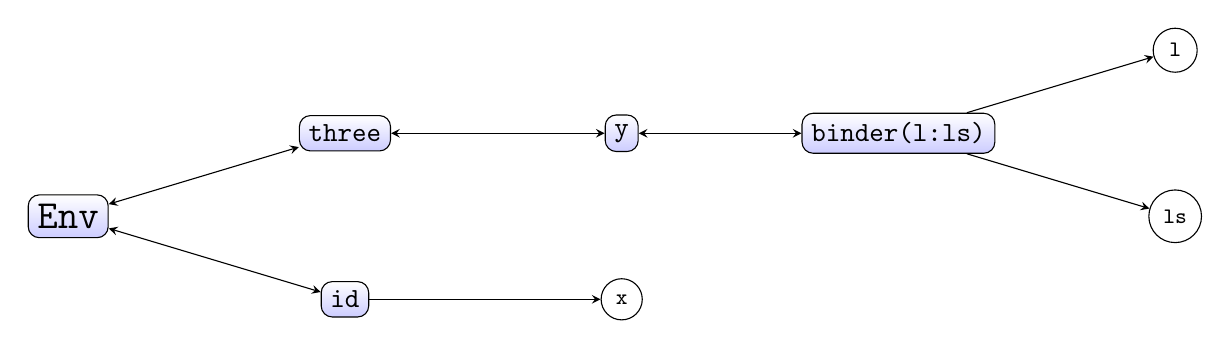
\begin{tikzpicture}
  [
    grow                    = right,
    sibling distance        = 6em,
    level distance          = 10em,
    edge from parent/.style = {draw, -latex, >=stealth},
    every node/.style       = {font=\footnotesize},
    sloped
  ]
  \node [root] {Env}
    child { node [env] {id}
         child { node [dummy] {\texttt{x}}
              edge from parent [->] node [below] {} } 
         edge from parent [<->] node [below] {} }
    child { node [env] {three}
         child { node [env] {\texttt{y}}
             child { node [env] {\texttt{binder(l:ls)}}
               child { node [dummy] {\texttt{ls}}
                         edge from parent [->] node [above] {}  }
               child { node [dummy] {\texttt{l}}
                         edge from parent [->] node [below] {} }
             edge from parent [<->] node [below] {} }
         edge from parent [<->] node [below] {} } 
    edge from parent [<->] node [below] {} };
\end{tikzpicture}
  }
\caption{Scope and class hierarchy, blue boxes are classes, and white circles are
references to variables, then arrows signify a reference to the object
being pointed to in the object which the arrow stems.}
\label{figure:scope_map}
\end{figure}

The top level functions of the program will be stored in an \verb|Env| class, then each
possibly mutually recursive function will have a reference to every other function, via the \verb|Env| class.

\subsection{CoreExpr Constructs}
\begin{itemize}
\item The \texttt{Lit} construct will be represented as either a
\texttt{CharThunk} or an \texttt{IntThunk} containing the value
of the literal.

\item The \texttt{Var} construct will either be a build in function, 
in which case it will be thunk when evaluated will return the build-in
value. 

\item The \verb|Lam b e| construct will generate the following
code in a separate class file:
\begin{JavaLst}
public class &\textit{NAME}& implements Function {
  &\textit{ty}&(&\textit{t}&) arg;
  &\textit{Parent}& p;
  &\textit{NAME}& (&\textit{Parent}& p) {
    this.p = p
  }

  protected &\textit{ty}&(&\textit{e}&) (&\textit{ty}&(&\textit{b}&) arg) {
    this.arg = arg
    return &$\llbracket \textit{e} \rrbracket$&.get();
  }
}
\end{JavaLst}
\textit{NAME} will be the unique name of the function.
\textit{ty} will return the Java type of the either the binder \texttt{b}
or the expression in the lambda \texttt{e} and $\llbracket \texttt{e} \rrbracket$ is a sequence
of expression produced by converting \texttt{e} to a JVM bytecode.

The code snipped returned will create a function object for this function
and then wrap it inside a thunk. This is the Java implementation of 
translation relation above.

\begin{JavaLst}
new ObjThunk(new &\textit{Name}&(&\textit{Parent}&));
\end{JavaLst}

\item The \verb|App| mapping first creates a class which represents the thunk for 
  \verb|App e1 e2|, 

\begin{JavaLst}
public class &\textit{AppName}& implements Thunk {
  &\textit{Parent}& p;
  &\textit{NAME}& (&\textit{Parent}& p) {
    this.p = p
  }

  public force() {
    return (Supplier)(&$\llbracket e_1 \rrbracket$&.get()).apply(&$\llbracket e_2 \rrbracket$&);
  }
}
\end{JavaLst}
Then the returned source code is 

\begin{JavaLst}
new &\textit{AppName}&(&\textit{Parent}&);
\end{JavaLst}

\item \verb|Let| is just mapped to \verb|Lam| and then converted to JVM bytecode in the same
  way that \verb|Lam| is.

\item \verb|Case| is mapped to a sequence of conditions where the case binder is checked again the 
  value being scrutinised. There are examples in 
  Appendix~\ref{appendix:bytecodetranslationdoc}

\end{itemize}

\section{Runtime Library}

There is a small runtime library included with JVHC, this library is implemented in Java code.
This allowed for arbitrary side effect free Java code to invoked by Haskell code. 
The JVHC compiler must also be made aware of the type and Java name of each of the functions exposed from 
the Java world. The runtime is bundled in the package \verb|BuildIn|, and includes for example
a function to add two integers.

\subsection{I/O Monad}

Haskell, as mentioned previously, is a pure language without side effects. If Haskell
is to allow I/O or any possible side effect, then this can be implemented using an I/O
monad abstraction. The I/O monad represents a sequence of instructions that when run will result in 
the sequence of value being executed in order. The I/O monad can only be run by the runtime
of the program. This happens when the I/O monad is returned from the executing code
to the \verb|main| function at which point the runtime will force evaluation of the monad,
since Haskell program itself never start the computation purely of functions is preserved even
with the I/O monad.
Then code like this can be written which will read continuously read a value and print out $2\times$ that
value
\begin{HaskellLst}
times2 :: IO Int
times2 = getInt >>= (\i -> putInt (i*2) >> times2)
\end{HaskellLst}
There are three thing to explain. \verb|getInt :: IO Int| create a computation that when called 
will return a \verb|IO Int|, then represents the computation that when run 
\verb|putInt :: Int -> IO ()| will take an int value and print it to the screen. Then 
\verb|>>= :: IO a -> (a -> IO b) -> IO b| (pronounced bind) is used to combine monads.
The type of \verb|>>=| is interesting, it allow access to the value inside the monad (this is 
useful since at the current point of execute the value which will be passed to the function may 
still not be know). Then \verb|>>| is similar to \verb|>>=| put ignoring the result of the 
first monad.
The I/O monad is implemented as a Java interface
\begin{JavaLst}
public interface IO<R> { R unsafePerformIO(); }
\end{JavaLst}
Then in the runtime will call \verb|unsafePerformIO| on the return value of the \verb|main|
function.


\section{Benchmarking}

\begin{itemize}
  \item Talk about fully evaluating expression in Haskell, not just
    weak head normal form.

  \item Talk about Criterion for simple Haskell benchmarks.

  \item Talk about how the benchmarker was implemented to test
    multiple run of compiled Haskell program. Could talk
    about Haskell system programming.

  \item 
\end{itemize}

\end{document}
